\documentclass[11pt,a4wide]{article}
\usepackage{verbatim}
\usepackage{listings}
\usepackage{graphicx}
\usepackage{a4wide}
\usepackage{color}
\usepackage{amsmath}
\usepackage{amssymb}
\usepackage[dvips]{epsfig}
\usepackage[T1]{fontenc}
\usepackage{cite} % [2,3,4] --> [2--4]
\usepackage{shadow}
\usepackage{hyperref}

\setcounter{tocdepth}{2}

\lstset{language=c++}
\lstset{alsolanguage=[90]Fortran}
\lstset{basicstyle=\small}
\lstset{backgroundcolor=\color{white}}
\lstset{frame=single}
\lstset{stringstyle=\ttfamily}
\lstset{keywordstyle=\color{red}\bfseries}
\lstset{commentstyle=\itshape\color{blue}}
\lstset{showspaces=false}
\lstset{showstringspaces=false}
\lstset{showtabs=false}
\lstset{breaklines}
\begin{document}
\section*{Introduction to numerical projects}

Here follows a brief recipe and recommendation on how to write a report for each
project.
\begin{itemize}
\item Give a short description of the nature of the problem and the eventual 
numerical methods you have used.
\item Describe the algorithm you have used and/or developed. Here you may find it convenient
to use pseudocoding. In many cases you can describe the algorithm
in the program itself.

\item Include the source code of your program. Comment your program properly.
\item If possible, try to find analytic solutions, or known limits
in order to test your program when developing the code.
\item Include your results either in figure form or in a table. Remember to
       label your results. All tables and figures should have relevant captions
       and labels on the axes.
\item Try to evaluate the reliabilty and numerical stability/precision
of your results. If possible, include a qualitative and/or quantitative
discussion of the numerical stability, eventual loss of precision etc. 

\item Try to give an interpretation of you results in your answers to 
the problems.
\item Critique: if possible include your comments and reflections about the 
exercise, whether you felt you learnt something, ideas for improvements and 
other thoughts you've made when solving the exercise.
We wish to keep this course at the interactive level and your comments can help
us improve it.
\item Try to establish a practice where you log your work at the 
computerlab. You may find such a logbook very handy at later stages
in your work, especially when you don't properly remember 
what a previous test version 
of your program did. Here you could also record 
the time spent on solving the exercise, various algorithms you may have tested
or other topics which you feel worthy of mentioning.
\end{itemize}



\section*{Format for electronic delivery of report and programs}
%
This project counts 1/3 of the final mark. The feedback will, in addition to our comments contain a final score, where 100 is the maximum. Project 4 counts also 1/3 of the final mark. The final exam stands for the remaining 1/3 of the final mark.
We have set up devilry so that you can use your candidate number only. Please mark your project with the candidate number. If you prefer to not use the candidate number, we will need it anyway in order to correlate with the final written exam. 

The preferred format for the report is a PDF file. You can also
use DOC or postscript formats or as an ipython notebook file. 
As programming language we prefer that you choose between C/C++, Fortran2008 or Python.
The following prescription should be followed when preparing the report:
\begin{itemize}
\item Use Devilry to hand in your projects, log in  at 
\url{ http://devilry.ifi.uio.no} with your normal UiO username and password
and choose either 'fys3150' or 'fys4150'. This time however you should use your candidate number only. You are free to use your name as well, but we need the candidate number for the final mark. 
\item You can upload the report file as well as your program files to devilry!  For the source code file(s) you have developed you can also place these at  a github domain, or eventually upload all program files to devilry.  
The report file should include all of your discussions and a list of the codes you have developed. 
\item You should include tests and/or unit tests of your code(s).
\item Comments  from us on your projects, with final score
will be available under
your Devilry domain and are only visible to you and the teachers of the course.

\end{itemize}

Finally, even though this project counts 1/3 of the final mark, 
we encourage you to work two and two together. Optimal working groups consist of 
2-3 students. You can then hand in a common report. 


\section*{Project 5, Astronomy project, $N$-body simulation of an open galactic cluster, deadline  Friday December 4}




The goal in this project is to develop a code that can perform simulations of an
open cluster using Newtonian gravity. First, however we will compare
the stability of two different methods. This is because when we are
looking at a system with a large number of particles, we are more
interested in the statistical properties of the system than in the
individual motion of each of the particles. This means that the
stability of the solution method is more important than its short term
accuracy.  This project is inspired by an article by Joyce {\em et al.}, see Ref.~\cite{joyce2010} below.
When  solving this project, we recommend downloading this article. It is a good companion to understand the 
physics discussed here. 

In the first part of this project we will explore the stability of two
well-tested numerical methods for solving differential equations. The algorithms to test and implement are the fourth-order Runge-Kutta method and the Velocity-Verlet method. 

\begin{enumerate}
\item[a)] Implement the Newtonian two-body (you can choose masses and dimensionalities as
  you wish) problem in three dimensions using the fourth order
  Runge-Kutta method and the Velocity-Verlet method discussed in
  the lecture notes.

 Compare the
stability of the two different methods. How do they work for large
time steps? How do they work for very long times? Compare also the
time used to advance one timestep for the two different
methods. Comment your results. Which algorithm would you use for
simulating systems that require long  times?

\end{enumerate}





We will now try to build a simple model of an open
cluster, see Ref.~\cite{openclusterref}. An
open cluster is a group of up to a few thousand gravitationally bound
stars created from the collapse of a molecular cloud. This collapse
leads to a flurry of star formation. Open clusters are usually found
in the arms of spiral galaxies, or in irregular galaxies. Since stars
in an open cluster have roughly the same age, and are made from the
same material, they are interesting in the study of stellar evolution,
since many of the variable parameters we have when comparing two stars
are kept constant.

Once open clusters are formed they gradually dissipate as members get
ejected from the cluster due to random collisions, this means that
open clusters generally last only a few hundred million years. In
figure \ref{HR}, we see the Hertzsprung-Russell diagrams for two open
clusters.

\begin{figure}[!h]
\centering
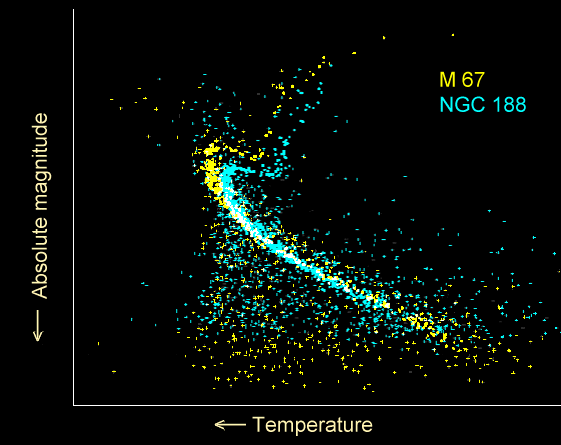
\includegraphics[width=10cm]{FigAstro/open_cluster_hr_diagram_ages.png}
\caption{Hertzsprung-Russell diagrams for two open clusters, M67 and
  NGC 188. We see that most of the stars are on the main sequence. In
  the older cluster, NGC 188, we see that the heaviest stars are just
  now leaving the main sequence, while the younger cluster, M67, is
  following closely after.}
\label{HR}
\end{figure}

We will look at a simple model for how an open cluster is made from
the gravitational collapse and interaction among a large number of
stars. We want to study this collapse, and the statistical properties
of the collapsed system.

One particle in our model represents one or a few stars, and we will
work first with a few hundred particles. We will simulate what is called a
``cold collapse'', this means that we start the particles with little
or no initial velocity.
\begin{enumerate}
\item[b)] Extend your code to an arbitrary number of particles, $N$,
  starting with a uniform (random) distribution within a sphere of a
  given radius $R_0$. Start the particles at rest, with masses
  randomly distributed by a Gaussian distribution around ten solar
  masses with a standard deviation of one solar mass. Use solar masses
  and light years as units of mass and length and make your equations dimensionless.
The function {\em GaussPDF} included with this project can be used to generate 
random numbers which follow a Gaussian (or normal) distribution.  The function for calculating these random numbers can be found at the webpage of the course together with the project files.

How large time steps are required given $R_0 = 20 ly$
(light years), and a $N = 100$? Do we have any units of time that fit
this timescale?   
In the limit where $N \rightarrow \infty$, keeping $\rho_0$ constant,
we get a continuous fluid. In this case the system collapses into a
singularity at a finite time $\tau_{crunch} = \sqrt{\frac{3\pi}{32G\rho_0}}$. 
(For the especially interested (Not required!): Can
you derive this result? Hint: recall the Friedman equations \cite{friedmaneqs}).

Why do we not observe this singularity in our model? Use
$\tau_{crunch}$ as the unit of time, and find $G$ in these units ($G$
will become a function of the number of particles $N$, and the average
mass of the particles, $\mu$).

You should run these calculations with both the fourth-order Runge-Kutta algorithm
and the Velocity-Verlet method. Which method would you prefer? Give a critical discussion.

For the remaining exercises, you should use only one of the above methods. 

\item[c)] Run the system for a few $\tau_{crunch}$. Save the positions
  of the particles at different times to file. Does the system
  reach an equilibrium? How long time does this take ?

\item[d)] Make a function that calculates the kinetic and potential
  energy of the system. Is the energy conserved? Some of the
  particles are ejected from the system, how can we identify these
  particles from the energies we have calculated? How much of the
  energy of the system is taken away by particle ejection? How does
  this change with different values of $N$? Are there still particles
  being ejected after the system reaches equilibrium?


\item[e)] We will now introduce a smoothing function to take care of
  the numerical instability that arises when two of the particles come
  very close. There are a lot of ways of inserting such a smoothing, but
  we will just look at a very simple one. We will modify the Newtonian
  force law to make it finite at short ranges
\[ F_{mod} = -\frac{GM_1M_2}{r^2 + \epsilon^2}.\]

The parameter $\epsilon$ is a ``small'' real constant. What should the value of this parameter be? Try out different values (which one gives you the best energy conservation?). Can we justify this correction to the pure Newtonian force by noting that our particles do not represent actual point particles
but rather mass distributions of some finite extent? Does the addition
of this correction change any of the results from part e) ?


\item[f)] Now we will look at the particles that are bound (not
  ejected). What is the distribution of potential and kinetic energy?

The virial theorem says that for a bound gravitational system in
equilibrium we have
\[
2\langle K\rangle = -\langle V \rangle,
\] 
where $\langle K\rangle$
is the average (over time) kinetic energy of the system and $ \langle V
\rangle$ is the average potential energy. 

By the ergodic hypothesis we can take an ensamble average (average over a large system) instead of the time average. 

Are your results consistent with the virial theorem? 

\item[h)]  Try to plot the radial density of the particles (the particle density as a function of radius) in the
  equilibrium state. How would you extract such an information from your calculations? (Hint: make a histogram for the radial
particle density) What is the average distance? What is the
  standard deviation? Plot the radial distribution of particles.

Run the code for different number of initial particles, keeping the
total mass constant. \footnote{The interpretation of one particle as one or a few stars will not be useful any more when you increase the number of particles beyond a few thousand, however the analysis of gravitationally bound systems of many particles have much broader applications than cold collapse of open clusters, so the results are still highly relevant.} What is the average distance from the centre of the cluser as a function of $N$?

The radial distribution of particles in this kind of cold collapse can often be fit very well with the simple expression 
\[ 
n(r) = \frac{n_0}{\left(1 +\left(\frac{r}{r_0}\right)^4\right)}.
\]
Try to fit your data to this curve, what is the value $n_0$ and $r_0$? Can you find how these values depend on N?

How many particles can you simulate?

Compare your results with those found in Ref.~\cite{joyce2010}. 

If you want, you can also compare your results to the well-known Navarro-Frenk-White profile
\[ 
\rho(r) = \frac{\rho_0}{\frac{r}{r_0}\left(1 +\frac{r}{r_0}\right)^2}.
\]
Does this fit better?

\end{enumerate}
\begin{thebibliography}{100} 
\bibitem{joyce2010} M.~Joyce, B.~Marcos, and F.~Sylos Labini, Cold uniform spherical collapse revisited, AIP Conf. Proc. 1241, 955 (2010); \url{http://dx.doi.org/10.1063/1.3462740} and arXiv1011.0614 (2011), 
\url{http://arxiv.org/abs/1011.0614}.
\bibitem{openclusterref} P.~J.~E. Peebles, \emph{{The Large-Scale Structure of the Universe}}, Princeton
  University Press, 1980. See also C.~Payne-Gaposchkin,  {\em Stars and clusters}, (Cambridge, Harvard University Press, 1979), or just \url{https://en.wikipedia.org/wiki/Open_cluster}. 
\bibitem{friedmaneqs} A.~Friedman,  {\em On the Curvature of Space},  General Relativity and Gravitation {\bf 31},  1991 (1999), or just \url{https://en.wikipedia.org/wiki/Friedmann_equations}.
\end{thebibliography} 
\end{document}







